\section{APPENDIX CHAPTER 3}\label{APPENDIX CHAPTER 3}

\subsection{About Side Effects in Computations}
\label{app-Chap3-About Side Effects in Computations}


In computer science, an operation, function or expression is said to have a side effect if it modifies some state variable value(s) outside its local environment, which is to say if it has any observable effect other than its primary effect of returning a value to the invoker of the operation. Source: [\href{https://en.wikipedia.org/wiki/Side_effect_(computer_science)}{Side effect in computer science}].\\

It is extremely important that computing operations do not cause side effects unintentionally. The programmer must be aware of side effects if imperative programming paradigm is implemented, where the application state flows from one function to the next. The unintended changes in state information are basically side effects. If the change is intended (deliberate) then it is not a side effect. \\

For example, a global variable "count\_total\_lines" is intended to be incremented every time a specific local function executes, then it is not a side effect. When a second local function executes, it is also intended that the global variable "count\_total\_lines" be incremented. This is not a problem. \\

The side effect problems may exist if the program implements many global variables that are inter-related to each other in computations. Since there are many variables involved, it will be difficult to track which variable values should change, and which should not change. This is where side effects may occur. For example, if by mistake successive executions of different functions do not happen in the order as designed, then side effects will definitely occur. One example in computer science that creates side effect is a race condition. It was said that side effects are not only limited to state manipulation, in fact, interacting with the I/O, database, log system, APIs and anything else that can be controlled, has a side effect. \\

It is known that the functional programming paradigm aims to minimize or eliminate side effects. The lack of side effects in functional programming makes it easier to do formal verification of a program. Formal verification means verifying that the function executes correctly, and the execution also produces the correct results. \\

In general programming, there are many ways to reduce and minimize the occurrence of side effects. Proper naming of variables that separates global from local variables is helpful. Having the program flow design to be fully structured definitely helps. Program flows that are unstructured or haphazard invites disaster, especially the occurrence of side effects. \\

In practice, most applications will combined the declarative and imperative programming paradigms. There is a fine balancing act between the declarative (what do to) and imperative (how to do) paradigms, with more a shift in the community towards declarative programming. \\

This appendix is not meant to provide an exhaustive analysis on side-effects, a good read on it is provided at the URL link [\href{https://thejs.dev/jmitchell/what-are-side-effects-and-what-you-can-do-about-them-jws}{What are side effects and what you can do about them (2020).}]. 




%% ==============================
\clearpage
\pagebreak

\subsection{Realtime Computing Environment}
\label{app-chap3-Realtinme Computing Environment}


The official title of this thesis is "\textit{Realtime interpolation of parametric curves with chord-error and feedrate constraints.}" The word "realtime" is the first word in the title and it deserves to be discussed.\\

To a lay person, realtime means happening now, happening currently or immediately, or as it is happening, or occurring at the current instance or not happening in past time, or not occurring in delayed time. These interpretations are all correct. However, the interpretation of realtime in computing is different. This work satisfies both the layman and technical computing interpretations of realtime. \\

In layman's interpretation for the algorithm in this work, realtime means that as soon as the computation of the next interpolated point is completed, the interpolation algorithm will immediately send signals to the CNC machine to make that specific move. The cycle repeats for the next interpolated point until it reaches the end of the curve. This is the realtime according to the layman's interpretation. \\

Technically, in computing, real time is a guaranteed level of computer responsiveness within a specified time constraint, usually milliseconds or microseconds, between an event and its response deadline. This time delay between an event and its response is termed as time latency or just latency. \\

Real-time or real time describes various operations in computing or other processes that must guarantee response times within a specified time (deadline), usually a relatively short time. A real-time process is generally one that happens in defined time steps of maximum duration and fast enough to affect the environment in which it occurs, such as inputs to a computing system. Realtime does not mean fast or happening now. Realtime means it must be done before its deadline.\\

\clearpage
\pagebreak

The generally accepted technical definition of realtime is provided at URL [\href{https://en.wikipedia.org/wiki/Real-time_computing}{Real-time Computing}]. Real-time computing (RTC) is the computer science term for hardware and software systems subject to a "real-time constraint", for example from event to system response. Real-time programs must guarantee response within specified time constraints, often referred to as "deadlines"  or "maximum latency". \\

The interpolation algorithm developed in this work runs on a Real-Time Operating System (RTOS) and so makes the word "realtime" in its title accurate. The realtime requirements for timing latency of the algorithm's execution must be satisfied. \\

The LinuxCNC-Axis software that drives the G-Code signals generated by the algorithm runs on a realtime operating system (RTOS). If it is a non-RTOS, LinuxCNC-Axis software can only simulate running G-codes but not actually driving the electrical signals to the CNC machine. This is the first part of realtime in this thesis. \\

The next question is about the timing latency of computers in this work that will drive the G-Code signals. The maximum latency or deadline in this work is the time between the event of sending the signal to the time the CNC motors respond with the appropriate move. The signal travel time along the electrical wires is not a problem, since it is about 80 percent of the speed of light (almost instantaneous). The realtime requirement here is about the timing capability of the computer in sending repeated signals (worst case duration between a signal and its next signal). Sending a signal is an event, so the time between successive signals is a measure of latency. This worst case latency must be guaranteed for the computer.\\ 

Are the computers in this work capable of guaranteeing worst case latencies or deadlines to be considered realtime? The answer is definitely yes. It is confirmed by actual measurements, in which the results and discussions are provided in this document in section Cyclictest for Computer Latency Measurements [\ref{app4-Cyclictest for computer latency measurements}].  

 
%% ==================================================
\clearpage
\pagebreak

\subsection{Cyclictest for computer latency measurements}
\label{app4-Cyclictest for computer latency measurements}

In computing community, the cyclictest application program is a standardized shared code test that is used universally to measure computer hardware latencies. The results are captured in a tabular data format and plotted on a histogram. Essentially, the cyclictest code measures latency of the combined effect of the hardware, the firmware, and the operating system. \\

Cyclictest accurately and repeatedly measures the difference between a thread's intended wake-up time and the time at which it actually wakes up in order to provide statistics about the system's latencies. Cyclictest is most commonly used for benchmarking realtime (RT) systems. It is one of the most frequently used tools for evaluating the relative performance of real-time systems. Source: [\href{https://wiki.linuxfoundation.org/realtime/documentation/howto/tools/cyclictest/start}{Linux Foundation Cyclictest}] \\ 

\noindent
The results of cyclictest measurements in microseconds (us) for 10 million cycles (30 minutes run) in this work are as follows: 

\begin{enumerate}
	\item PASSED as RTOS. Histogram [\ref{Histogram-Latency-HP-Laptop-01-Debian10-10million-cycles.pdf}] shows a maximum latency value 42 (us) for HP-Laptop-01, on OS Debian 10 Kernel: 4.19.0-25-rt-amd64. 
	
	\item FAILED as RTOS. Histogram [\ref{Histogram-Latency-HP-Laptop-01-Ubuntu20-10million-cycles.pdf}] shows a maximum latency value 431 (us) for HP-Laptop-01, on OS Ubuntu 20.04 LTS Kernel: 5.15.0-86-lowlatency. 

	\item PASSED as RTOS. Histogram [\ref{Histogram-Latency-HP-Laptop-02-Debian10-10million-cycles.pdf}] shows a maximum latency value 46 (us) for HP-Laptop-02, on OS Debian 10 Kernel: 4.19.0-25-rt-amd64. 

    \item FAILED as RTOS. Histogram [\ref{Histogram-Latency-HP-Laptop-02-Ubuntu20-10million-cycles.pdf}] shows a maximum latency value 872 (us) for HP-Laptop-02, on OS Ubuntu 20.04 LTS Kernel: 5.15.0-86-lowlatency. 
\end{enumerate}

In the four(4) CPU Latency Performance Summary data tables at 
[\ref{tab-Debian10 HP-Laptop-01 CPU Performance}], 
[\ref{tab-Ubuntu20 HP-Laptop-01 CPU Performance}], 
[\ref{tab-Debian10 HP-Laptop-02 CPU Performance}], and
[\ref{tab-Ubuntu20 HP-Laptop-02 CPU Performance}], we can see that the average latencies for each of the 8-CPU cores as 2 (us) for RTOS and 8 (us) for non-RTOS. It is not the average latency that determines the RTOS status but the value of the worst case or maximum latency. The lower value for latency the  better.

%% ==================================================
\clearpage
\pagebreak

%% \begin{landscape}
\begin{figure}
\caption{Histogram-Latency-HP-Laptop-01-Debian10-10million-cycles}
\label{Histogram-Latency-HP-Laptop-01-Debian10-10million-cycles.pdf}
\centering
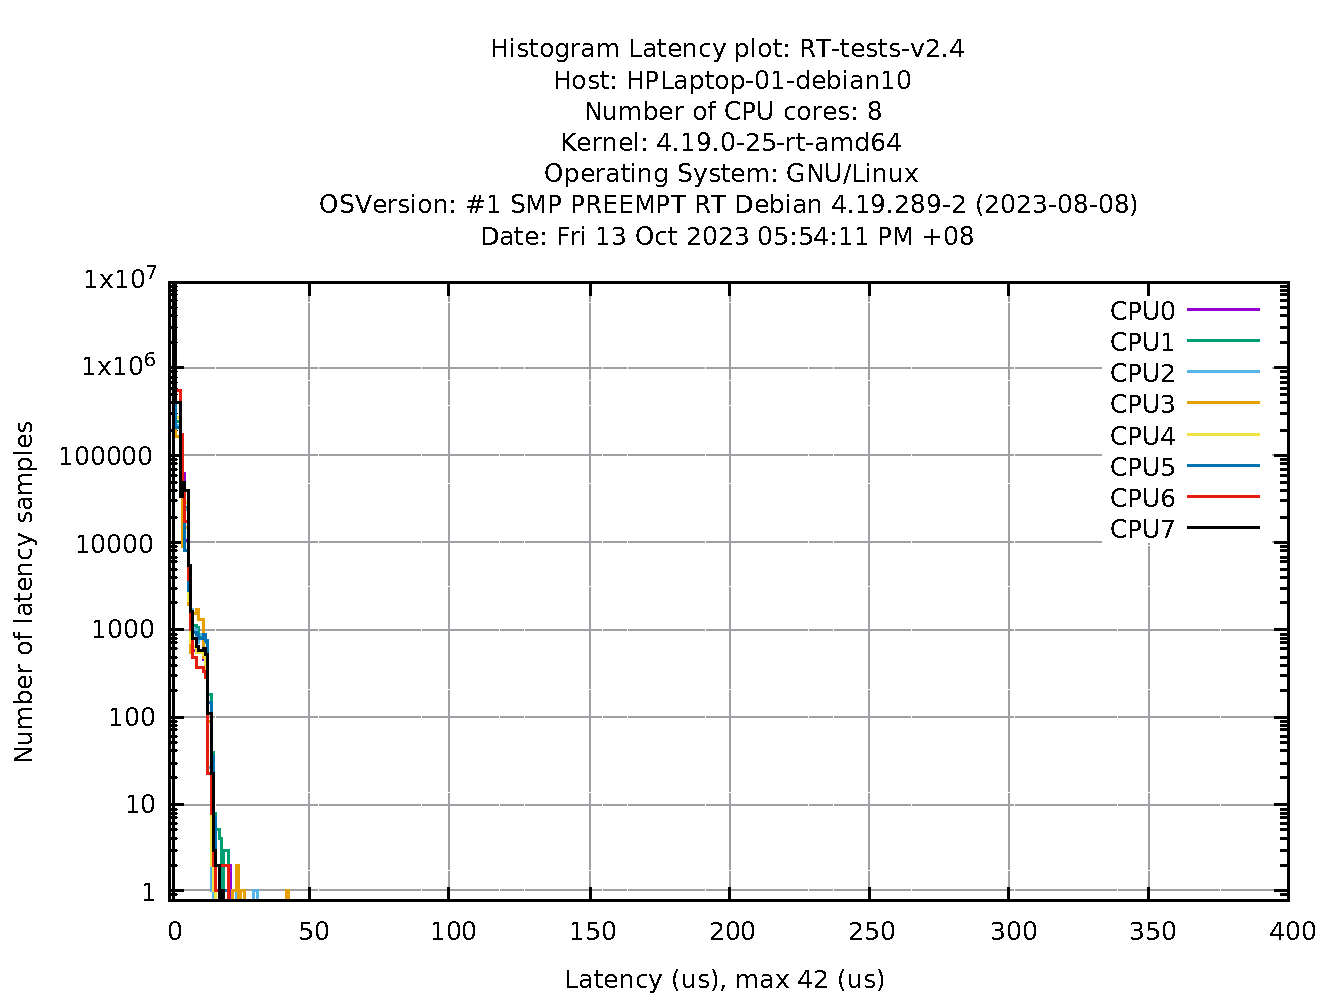
\includegraphics[width=1.00\textwidth]{Chap3/app-realtime/Histogram-Latency-HP-Laptop-01-Debian10-10million-cycles.pdf} 
\end{figure}	
%% \end{landscape}

\begin{figure}
\caption{Histogram-Latency-HP-Laptop-01-Ubuntu20-10million-cycles}
\label{Histogram-Latency-HP-Laptop-01-Ubuntu20-10million-cycles.pdf}
\centering
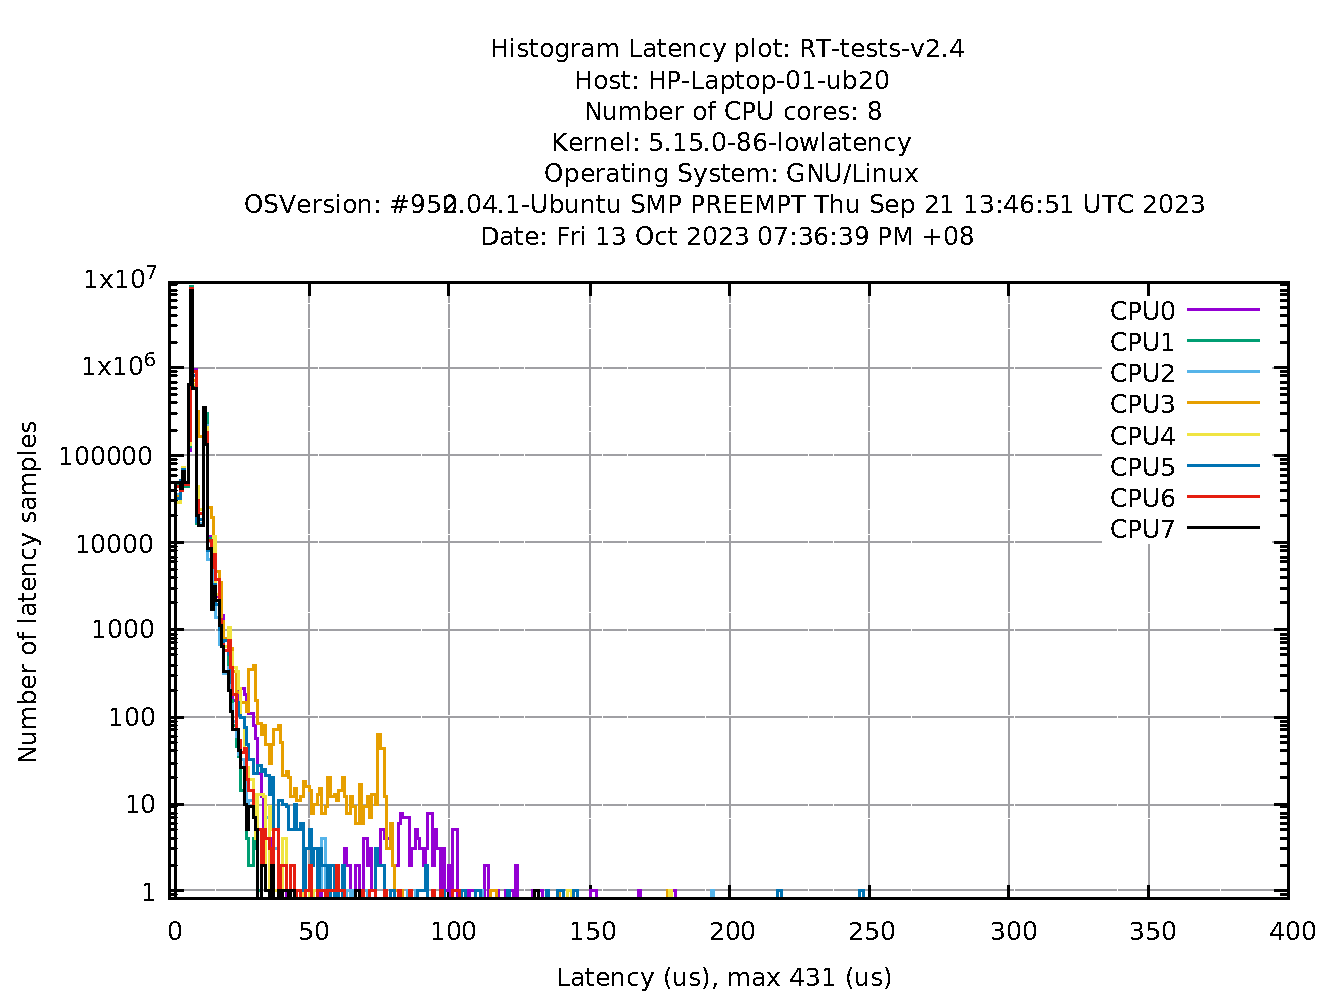
\includegraphics[width=1.00\textwidth]{Chap3/app-realtime/Histogram-Latency-HP-Laptop-01-Ubuntu20-10million-cycles.pdf} 
\end{figure}	

%% ==================================================
\clearpage
\pagebreak

\begin{figure}
\caption{Histogram-Latency-HP-Laptop-02-Debian10-10million-cycles}
\label  {Histogram-Latency-HP-Laptop-02-Debian10-10million-cycles.pdf}
\centering
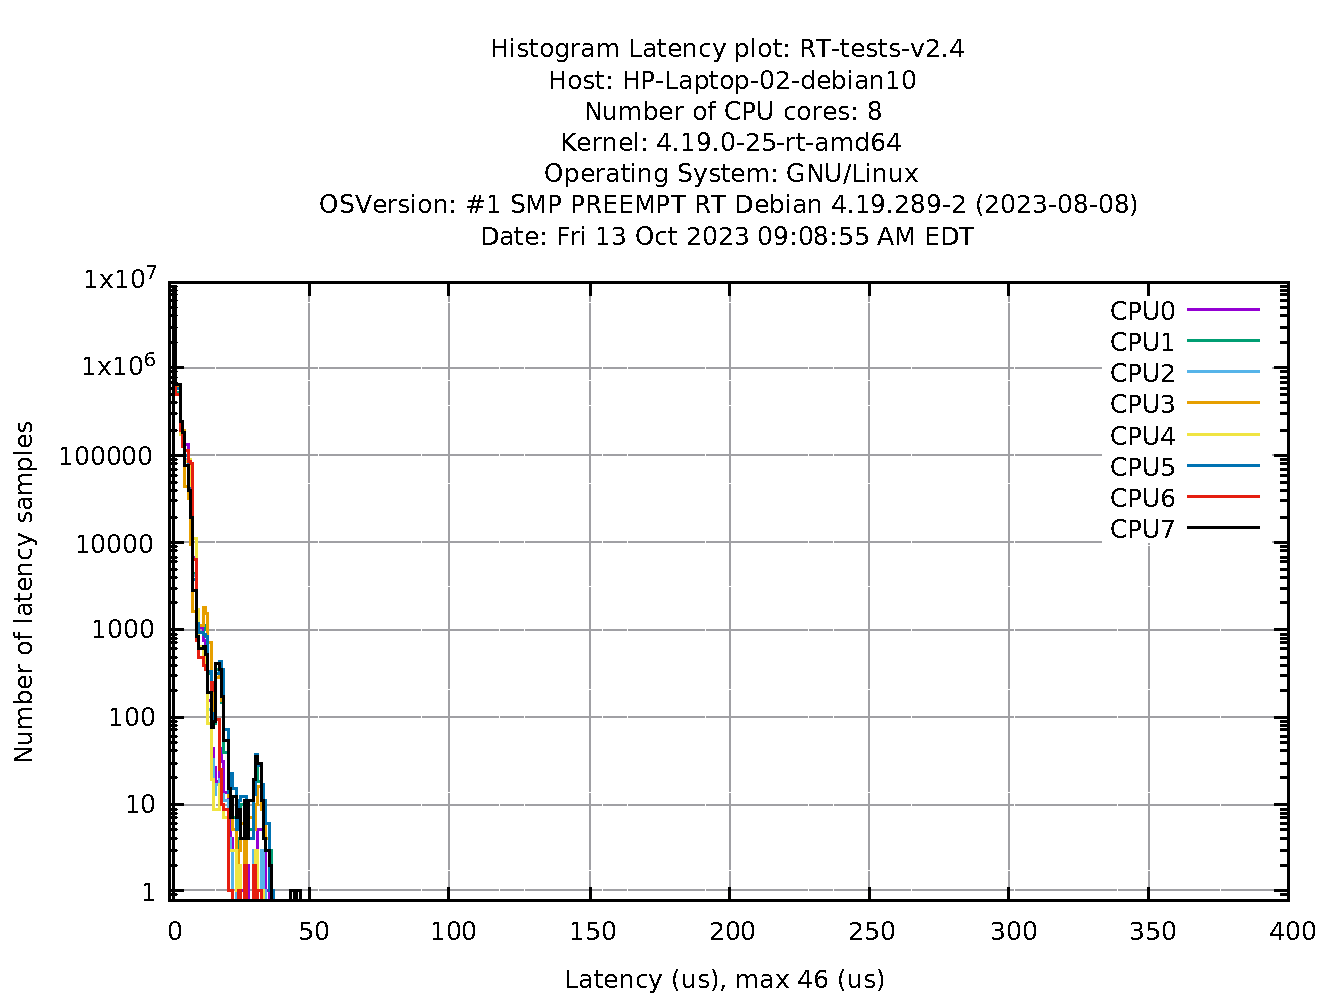
\includegraphics[width=1.00\textwidth]{Chap3/app-realtime/Histogram-Latency-HP-Laptop-02-Debian10-10million-cycles.pdf} 
\end{figure}	

\begin{figure}
\caption{Histogram-Latency-HP-Laptop-02-Ubuntu20-10million-cycles}
\label  {Histogram-Latency-HP-Laptop-02-Ubuntu20-10million-cycles.pdf}
\centering
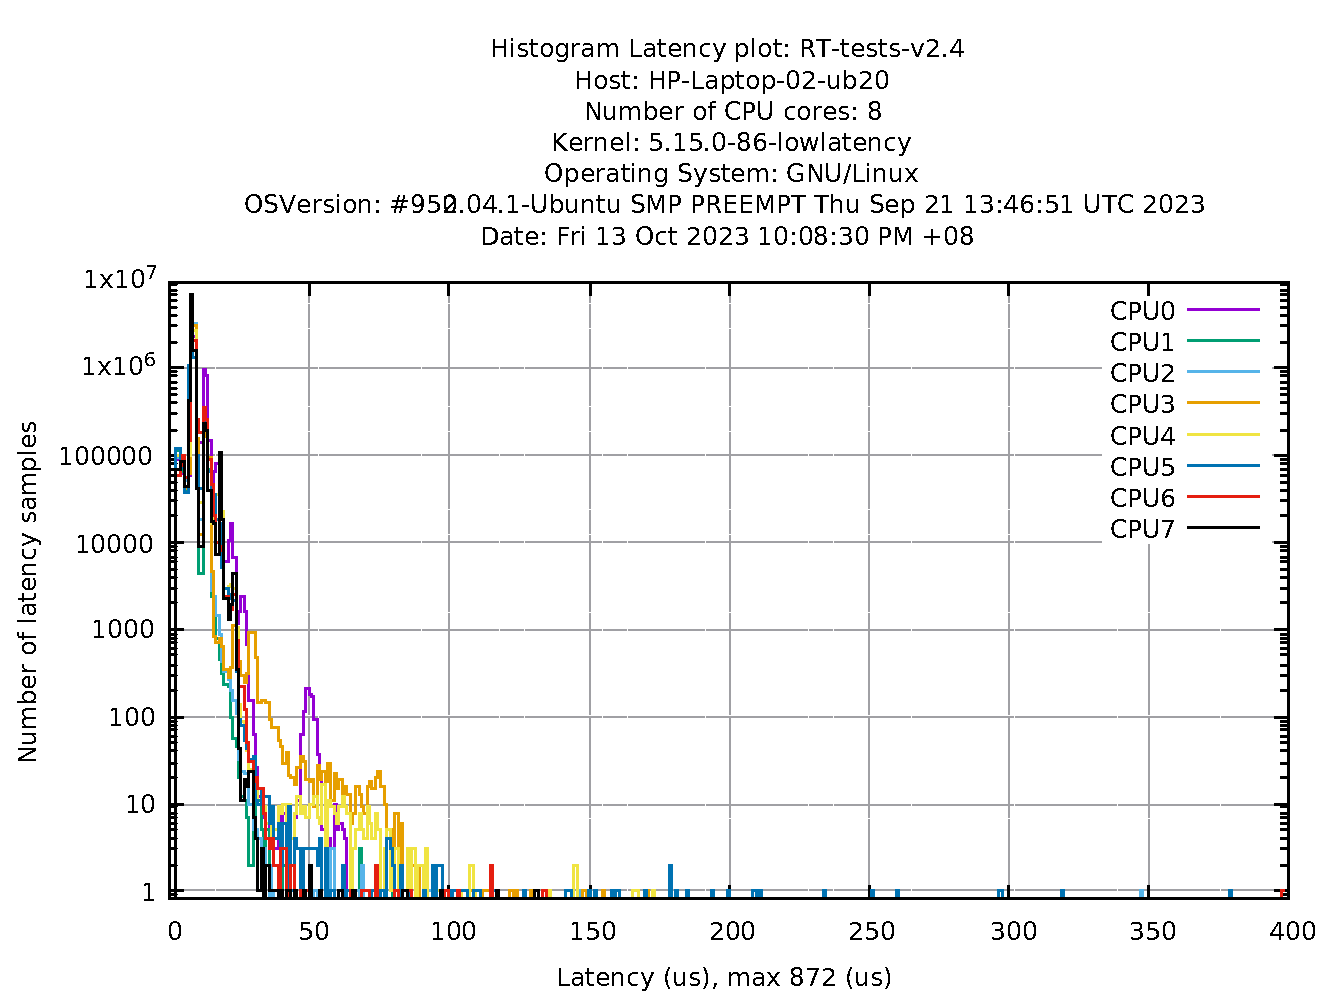
\includegraphics[width=1.00\textwidth]{Chap3/app-realtime/Histogram-Latency-HP-Laptop-02-Ubuntu20-10million-cycles.pdf} 
\end{figure}	


%% ==================================================
\clearpage
\pagebreak

\subsection{CPU Latency Performance Summary}

%% HP-LAPTOP-01-DEBIAN10 
\lstset{backgroundcolor=\color{white}, basicstyle=\linespread{0.92}\footnotesize, frame={topline, bottomline, leftline, rightline}}	
\begin{lstlisting}[caption={Debian10 HP-Laptop-01 CPU Performance}, label=tab-Debian10 HP-Laptop-01 CPU Performance]	
# Run for 10,000,000 cycles (approx 30 minutes)
# LATENCY (us)         CPU0  CPU1  CPU2  CPU3  CPU4  CPU5  CPU6  CPU7
# Min Latencies:       00002 00002 00002 00002 00002 00002 00002 00002
# Avg Latencies:       00002 00002 00002 00002 00002 00002 00002 00002
# Max Latencies:       00021 00020 00031 00042 00016 00020 00020 00019
# Histogram Overflows: 00000 00000 00000 00000 00000 00000 00000 00000
\end{lstlisting}

%% HP-LAPTOP-01-UBUNTU20 
\lstset{backgroundcolor=\color{white}, basicstyle=\linespread{0.92}\footnotesize, frame={topline, bottomline, leftline, rightline}}	
\begin{lstlisting}[caption={Ubuntu20 HP-Laptop-01 CPU Performance}, label=tab-Ubuntu20 HP-Laptop-01 CPU Performance]	
# Run for 10,000,000 cycles (approx 30 minutes)
# LATENCY (us)         CPU0  CPU1  CPU2  CPU3  CPU4  CPU5  CPU6  CPU7
# Min Latencies:       00003 00003 00003 00003 00003 00003 00003 00003
# Avg Latencies:       00008 00008 00008 00008 00008 00008 00008 00008
# Max Latencies:       00431 00040 00194 00178 00179 00247 00103 00131
# Histogram Overflows: 00001 00000 00000 00000 00000 00000 00000 00000
\end{lstlisting}

%% HP-LAPTOP-02-DEBIAN10 
\lstset{backgroundcolor=\color{white}, basicstyle=\linespread{0.92}\footnotesize, frame={topline, bottomline, leftline, rightline}}	
\begin{lstlisting}[caption={Debian10 HP-Laptop-02 CPU Performance}, label=tab-Debian10 HP-Laptop-02 CPU Performance]	
# Run for 10,000,000 cycles (approx 30 minutes)
# LATENCY (us)         CPU0  CPU1  CPU2  CPU3  CPU4  CPU5  CPU6  CPU7
# Min Latencies:       00002 00002 00002 00002 00002 00002 00002 00002
# Avg Latencies:       00002 00002 00002 00002 00002 00002 00002 00002
# Max Latencies:       00035 00037 00034 00036 00033 00037 00032 00046
# Histogram Overflows: 00000 00000 00000 00000 00000 00000 00000 00000
\end{lstlisting}

%% HP-LAPTOP-02-UBUNTU20 
\lstset{backgroundcolor=\color{white}, basicstyle=\linespread{0.92}\footnotesize, frame={topline, bottomline, leftline, rightline}}	
\begin{lstlisting}[caption={Ubuntu20 HP-Laptop-02 CPU Performance}, label=tab-Ubuntu20 HP-Laptop-02 CPU Performance]	
# Run for 10,000,000 cycles (approx 30 minutes)
# LATENCY (us)         CPU0  CPU1  CPU2  CPU3  CPU4  CPU5  CPU6  CPU7
# Min Latencies:       00003 00003 00003 00003 00003 00003 00003 00003
# Avg Latencies:       00009 00008 00008 00008 00008 00008 00008 00008
# Max Latencies:       00065 00093 00872 00200 00173 00379 00398 00131
# Histogram Overflows: 00000 00000 00002 00000 00000 00000 00000 00000
\end{lstlisting}

%% ==================================================
\clearpage
\pagebreak

